\documentclass[10pt, twocolumn, a4paper]{article}
\usepackage[utf8]{inputenc}
\usepackage[T1]{fontenc}
\usepackage{amsmath, amssymb}
\usepackage{graphicx}
\usepackage{geometry}
\usepackage{hyperref}
\usepackage{booktabs}
\usepackage{xcolor}
\usepackage{float}

% Margins
\geometry{top=2cm, bottom=2cm, left=1.5cm, right=1.5cm, columnsep=0.8cm}

\definecolor{primary}{HTML}{000000}
\hypersetup{colorlinks=true, linkcolor=primary, urlcolor=primary}

\begin{document}

% Full-width title + abstract
\twocolumn[{
\begin{center}
    {\Large\textbf{Economic Convergence Analysis using Bootstrap Methods}}\\[0.3em]
    {\large AppStats Project Report}\\[0.6em]
    \textbf{Loïc Huang} \\
    \href{mailto:Loic.Huang@eurecom.fr}{\texttt{Loic.Huang@eurecom.fr}} \\
    \small Student, EURECOM \\
    \small \textbf{Professor:} Motonobu Kanagawa
\end{center}
\vspace{0.4em}
\begin{center}
\fbox{\begin{minipage}{0.92\textwidth}
\small\textbf{Abstract.}
This project tests whether poor countries in 2000 grew faster than rich countries over
2000--2020, a pattern known as beta-convergence (Barro \& Sala-i-Martin, 1992).
We use GDP per capita data from Gapminder for 193 countries and split them into two groups
based on the global median income in 2000. We then compare their median log-growth rates
using a non-parametric bootstrap ($B = 2000$) to measure uncertainty. The observed difference
is $\hat{\theta} = 0.185$ (SE $= 0.053$), with a 95\% confidence interval of
$[0.081,\ 0.290]$. Since this interval does not include zero, the result supports the
convergence hypothesis.
\end{minipage}}
\end{center}
\vspace{1em}
}]

\section{Introduction}
The beta-convergence hypothesis says that poor countries tend to grow faster than rich ones.
The idea comes from basic economics: when a country has little capital, each new investment
brings a high return. As a country gets richer, returns on investment go down. This means
poor countries should grow faster and, over time, catch up with richer ones. This theory
was studied by Barro and Sala-i-Martin (1992).

\textbf{Our question:} Did countries that were below the global median income in 2000 grow
faster than richer countries between 2000 and 2020?

\section{Data and Variables}
We use GDP per capita from the Gapminder Data Portal. The values are adjusted for purchasing
power parity (PPP), which means the numbers account for differences in the cost of living
between countries. All values are in constant 2021 international dollars, so inflation does
not affect the comparison.

The dataset has 193 countries with complete data for both 2000 and 2020. We split them into
two groups using the global median GDP per capita in 2000 (\$9{,}351):
\begin{itemize}
    \item \textbf{Low-income group:} 96 countries below the median.
    \item \textbf{High-income group:} 97 countries at or above the median.
\end{itemize}
A more official split would use the World Bank income threshold (around \$12{,}000 in 2000),
which gives roughly 35 rich countries and 158 poor countries. However, such an unequal split
is not ideal for bootstrap: with only 35 countries in one group, the empirical distribution
approximates the true distribution less well, the median can only take a small number of
distinct values across replications, and the confidence interval becomes less stable. The
median split produces balanced groups of similar size, which gives more reliable bootstrap
estimates in both groups.

For each country $i$, we compute the log-growth rate over 20 years:
\begin{equation}
    g_i = \ln\!\left(\frac{\text{GDP}_{i,2020}}{\text{GDP}_{i,2000}}\right)
\end{equation}
We use the log-ratio instead of a simple percentage change because it is symmetric: a country
that doubles its GDP and a country that halves it get values of equal size with opposite signs.

\section{Estimation and Bootstrap}

\subsection*{Statistic of interest}
We use the median instead of the mean to compare the two groups, because some countries have
very extreme growth values (very high or very low) that would distort the mean. Our statistic is:
\begin{equation}
    \hat{\theta} = \text{median}(g_i \mid \text{poor}) - \text{median}(g_i \mid \text{rich})
\end{equation}

\subsection*{Why bootstrap?}
Computing $\hat{\theta}$ once is not enough. We need to know how uncertain this value is,
and in particular, whether zero is inside the 95\% confidence interval. If it is, the
difference we observe could just be random, and we cannot conclude anything about convergence.

The problem is that the median has no simple formula for its standard error. We therefore use
the non-parametric bootstrap to approximate the distribution of $\hat{\theta}$. We use
$B = 2000$ replications, which is enough to get stable estimates of the confidence interval bounds.

\subsection*{Algorithm}
For $b = 1, \ldots, B = 2000$:
\begin{enumerate}
    \item Draw a sample of size $n_{\text{poor}} = 96$ \textbf{with replacement} from the
          low-income group.
    \item Draw a sample of size $n_{\text{rich}} = 97$ \textbf{with replacement} from the
          high-income group.
    \item Compute: $\hat{\theta}^{*b} = \text{median}(\mathbf{g}^{*b}_{\text{poor}}) -
          \text{median}(\mathbf{g}^{*b}_{\text{rich}})$
\end{enumerate}

We resample \textit{within each group separately}. If we resampled from the full dataset
before the split, the median threshold would change at each step, moving countries between
groups. This would break the analysis, because we would no longer be measuring the same
comparison each time.

The standard error and confidence interval are then:
\begin{equation}
    \widehat{\text{SE}}_B = \sqrt{\frac{1}{B-1}\sum_{b=1}^{B}\!\left(\hat{\theta}^{*b} - \bar{\theta}^*\right)^2}
\end{equation}
\begin{equation}
    \text{CI}_{95\%} = \left[\hat{\theta}^{*(0.025)},\ \hat{\theta}^{*(0.975)}\right]
\end{equation}

\section{Results}

The median log-growth rate is $0.410$ for low-income countries and $0.225$ for high-income
countries, giving $\hat{\theta} = 0.185$. Figure~\ref{fig:eda} shows that the distributions
are right-skewed, which confirms why we use the median. The bootstrap gives a standard error
of $0.053$ and a 95\% confidence interval of $[0.081,\ 0.290]$ (Figure~\ref{fig:boot}).

\begin{figure}[H]
    \centering
    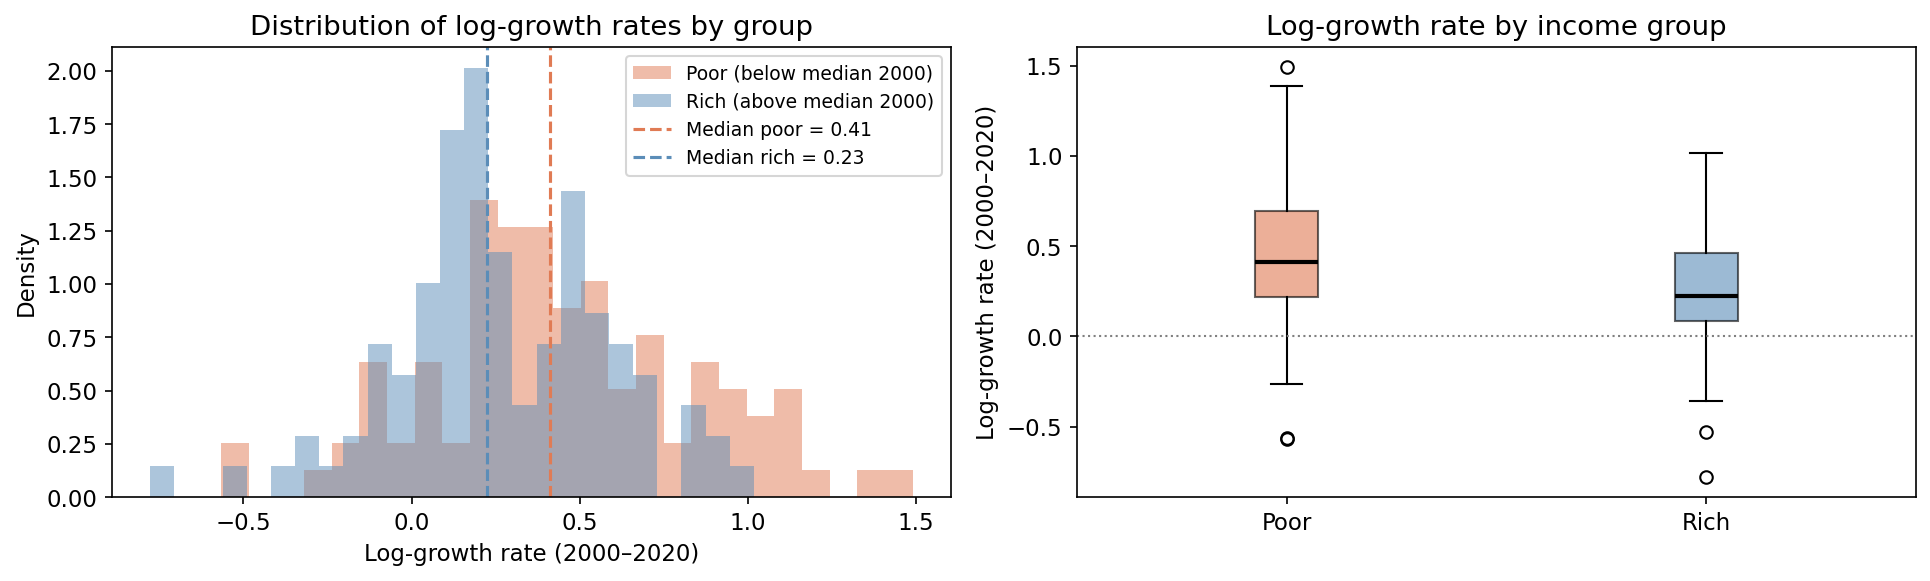
\includegraphics[width=\linewidth]{eda_growth_distributions.png}
    \caption{Log-growth rate distributions by group. Dashed lines show the group medians.}
    \label{fig:eda}
\end{figure}

\begin{figure}[H]
    \centering
    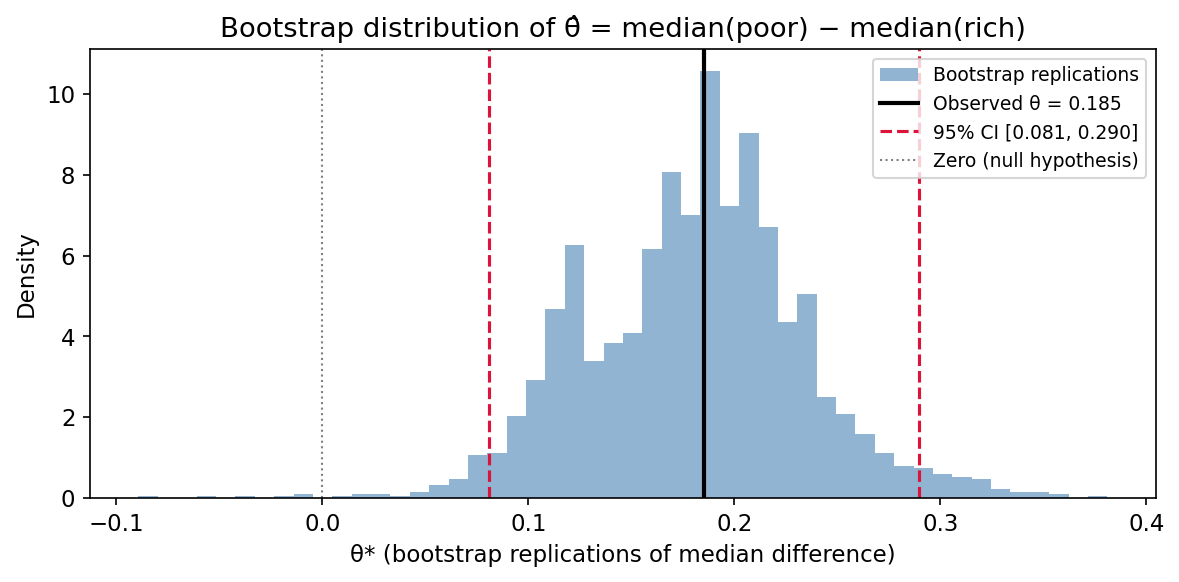
\includegraphics[width=\linewidth]{bootstrap_distribution.png}
    \caption{Bootstrap distribution of $\hat{\theta}$ ($B = 2000$). Red dashed lines: 95\%
    CI bounds. Grey dotted line: zero.}
    \label{fig:boot}
\end{figure}

\section{Interpretation}
The 95\% confidence interval $[0.081,\ 0.290]$ does not include zero. This means we can
reject the idea that the two groups grew at the same rate. Low-income countries in 2000 grew
significantly faster than high-income countries over 2000--2020, which is consistent with
the beta-convergence hypothesis.

However, this is a statistical \textit{association}, not a causal effect. Our analysis only
separates countries by their income in 2000. But poor and rich countries are different in
many other ways too, for example their institutions, education levels, or natural
resources. All of these factors also affect growth. So we cannot say that being poor
\textit{caused} faster growth. To show that, we would need to control for all these other
differences, for example using a multivariate regression. This is outside the scope of
this project.

Finally, the bootstrap relies on the empirical distribution $\hat{F}_n$ approximating the
true distribution $F$, which requires a large $n$. With 96 and 97 countries per group, this
approximation is reasonable in practice, but not perfect. The median is particularly sensitive
to this: with only 96 data points, the bootstrap median can only take a limited number of
distinct values, making the confidence interval bounds less precise than they would be with
a larger sample. This is a natural limit of the data: there are only 193 countries in
the world.

\end{document}
